\newpage
\section{3次元スロッシング}

数値解析例として矩形緒層内スロッシング解析を実施し、参考文献の結果と比較した。

\subsection{解析条件}

物性値パラメータを表\ref{table:3d-sloshing-material-property}に示す。流体は水と空気を仮定したパラメータである。
\renewcommand{\arraystretch}{1}
\begin{table}[H]
	\centering
	\caption{物性値}
	\begin{tabular}{ccccccc}
		\hline
		Test case & $\rho_1$ & $\rho_2$ & $\mu_1$ & $\mu_2$ & $\mathrm{g}$ \\
		\hline 
		Case$1$ & $1000$ & $1.2$ & $1.0e-3$ & $1.8e-5$ & $9.8$ \\
		\hline         
	\end{tabular}
	\label{table:3d-sloshing-material-property}
\end{table}
\renewcommand{\arraystretch}{1.0}

解析パラメータを表\ref{table:3d-sloshing-parameter}に示す。メッシュの細かさの違う条件で解析し、精度検証した。
\renewcommand{\arraystretch}{1}
\begin{table}[H]
	\centering
	\caption{解析パラメータ}
	\begin{tabular}{cccccc}
		\hline
		Test case & $\Delta t$ & メッシュ幅$dx$ & 界面幅$D$ & 再初期化回数 & 再初期化$\Delta \tau$\\
		\hline 
		Case$1$ & $0.0025$ & $0.025$ & $0.075$ & $5$ & $0.0001$\\
		Case$2$ & $0.0010$ & $0.010$ & $0.030$ & $5$ & $0.0001$\\
		\hline         
	\end{tabular}
	\label{table:3d-sloshing-parameter}
\end{table}
\renewcommand{\arraystretch}{1.0}

解析領域は幅$1.0\mathrm{m}$、奥行き$0.2\mathrm{m}$、高さ$1.2\mathrm{m}$であり、水が高さ$0.5\mathrm{m}$まで入っている状態である。
境界条件は全壁面でスリップ条件を与えた。
メッシュは六面体1次要素で、節点数18,081、要素数15,360である。

\begin{figure}[H]
	\centering
	\begin{minipage}[b]{0.49\columnwidth}
	    \centering
	    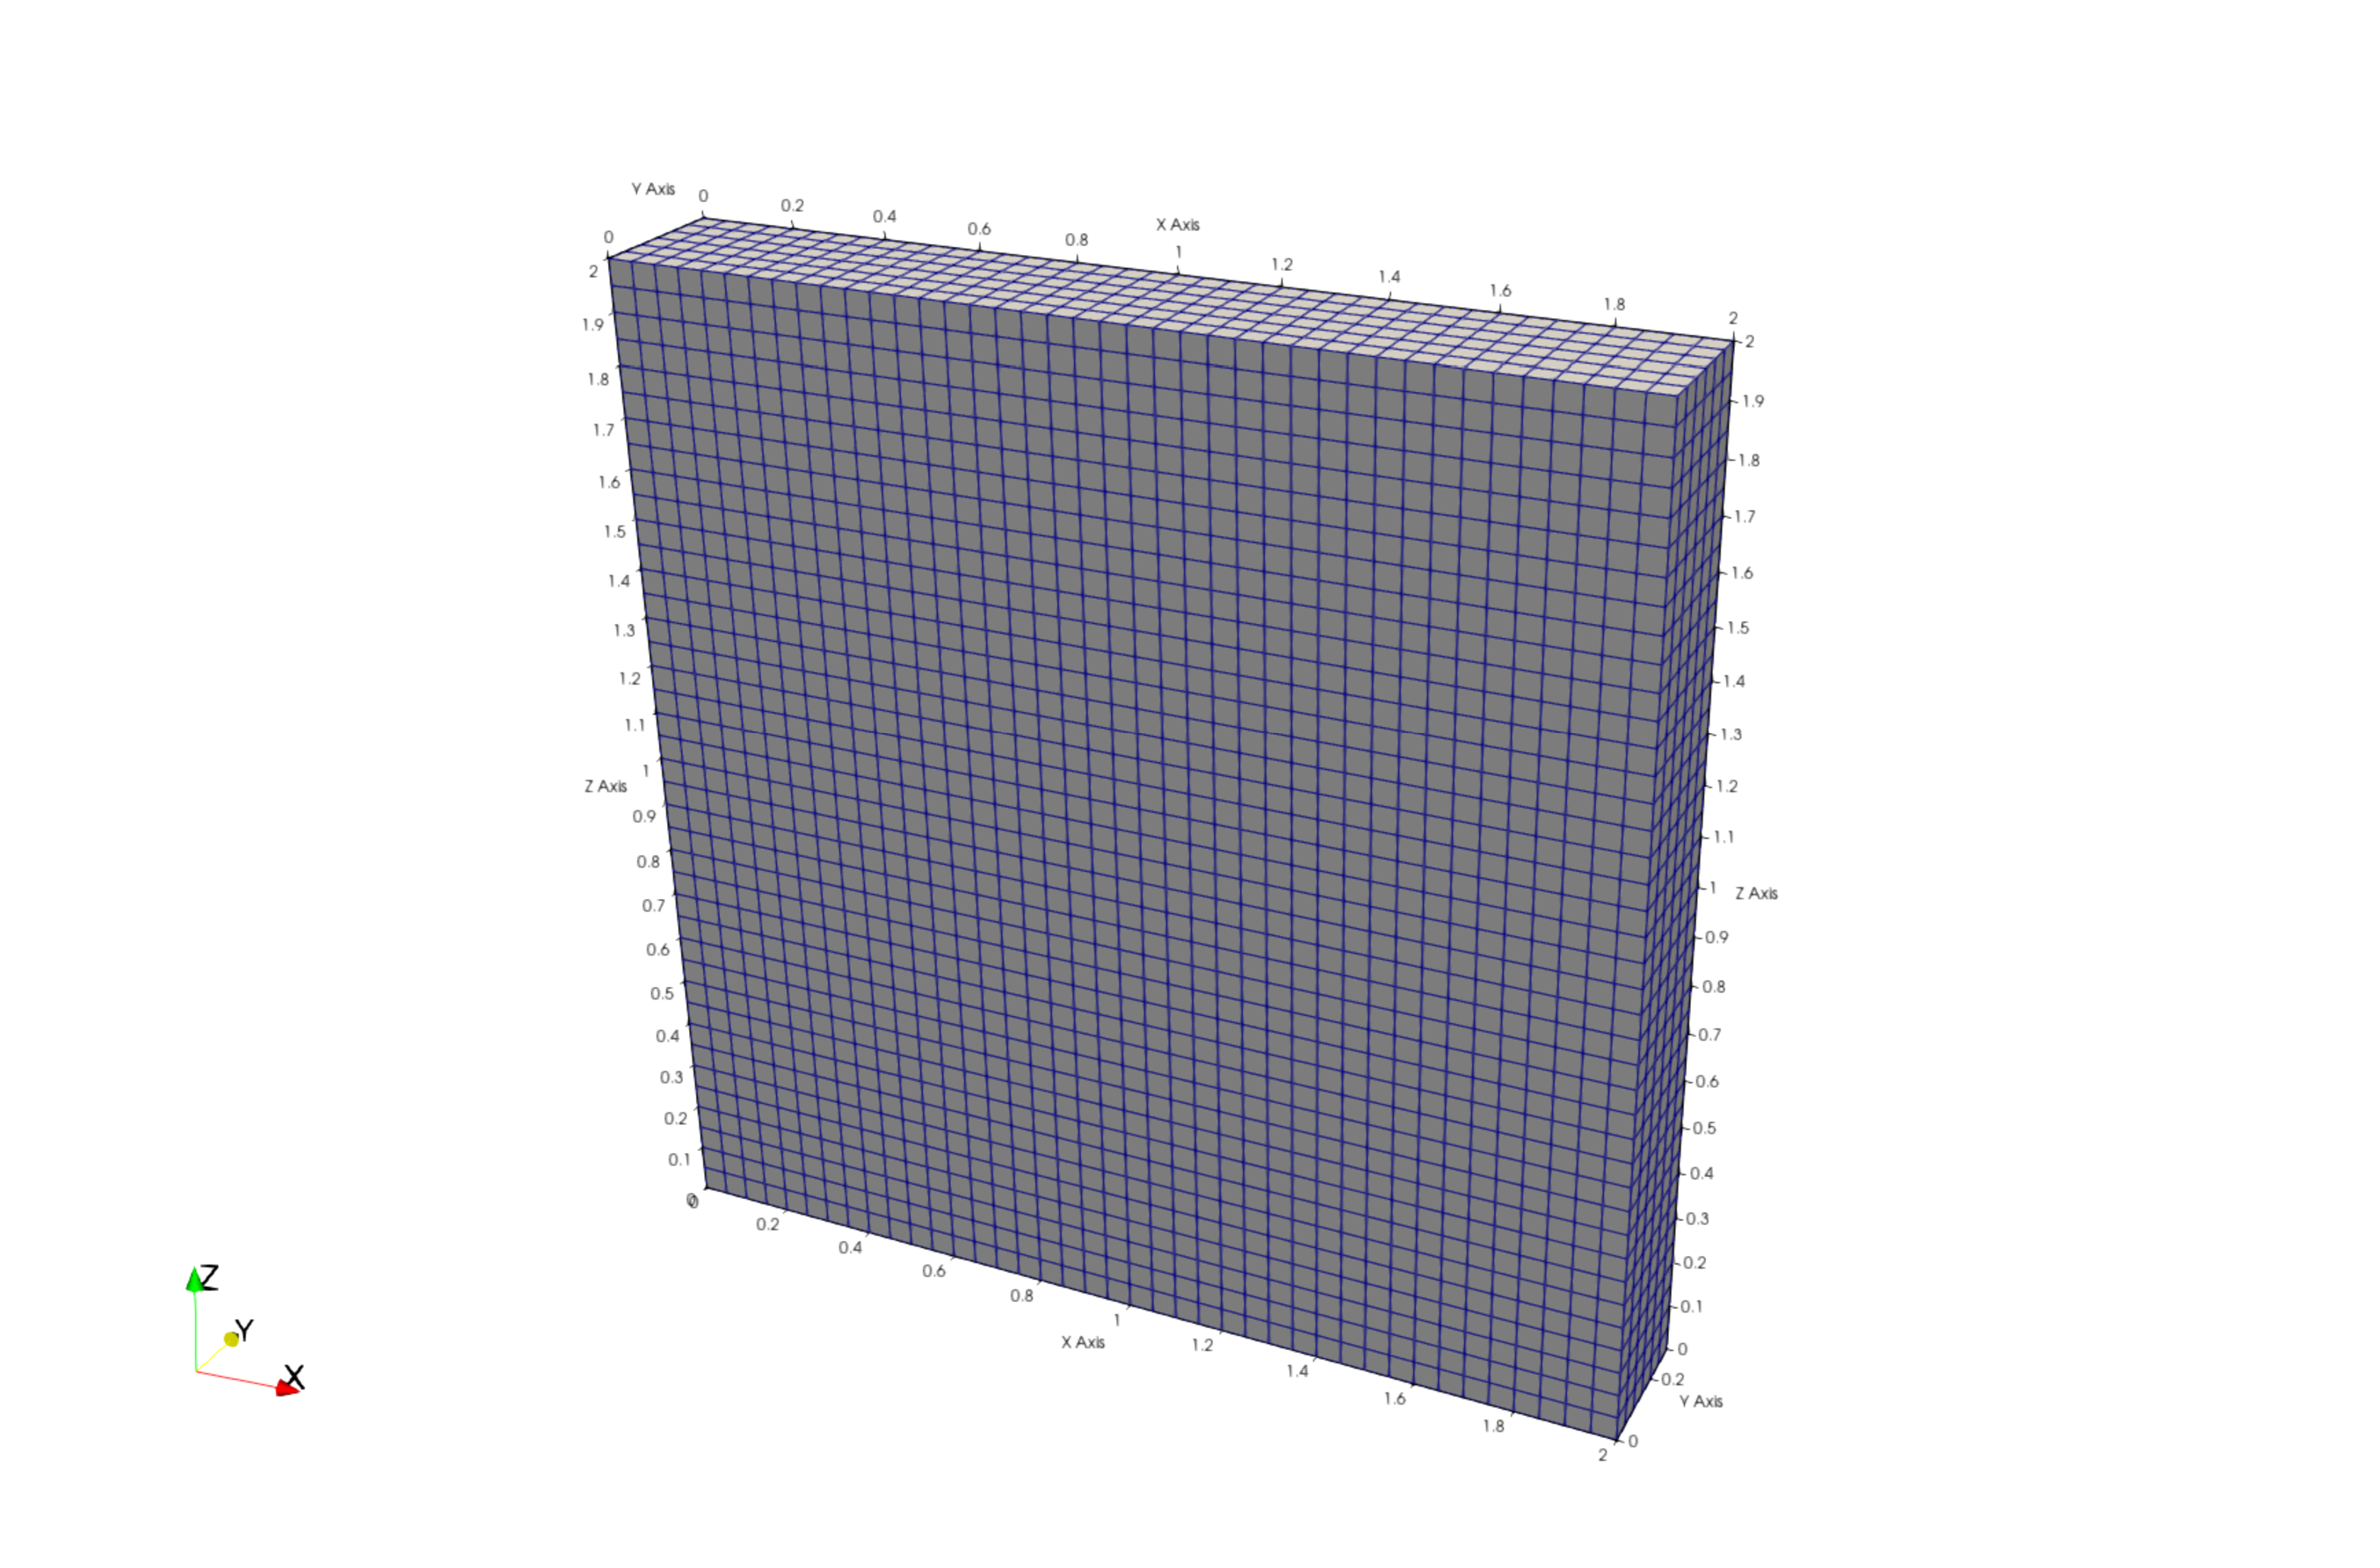
\includegraphics[width=6truecm]{pics/3d-sloshing/mesh.jpeg}
		\caption{3次元スロッシングの計算メッシュ}
		\label{fig:3d-sloshing-mesh}
	\end{minipage}
	\begin{minipage}[b]{0.49\columnwidth}
	    \centering
	    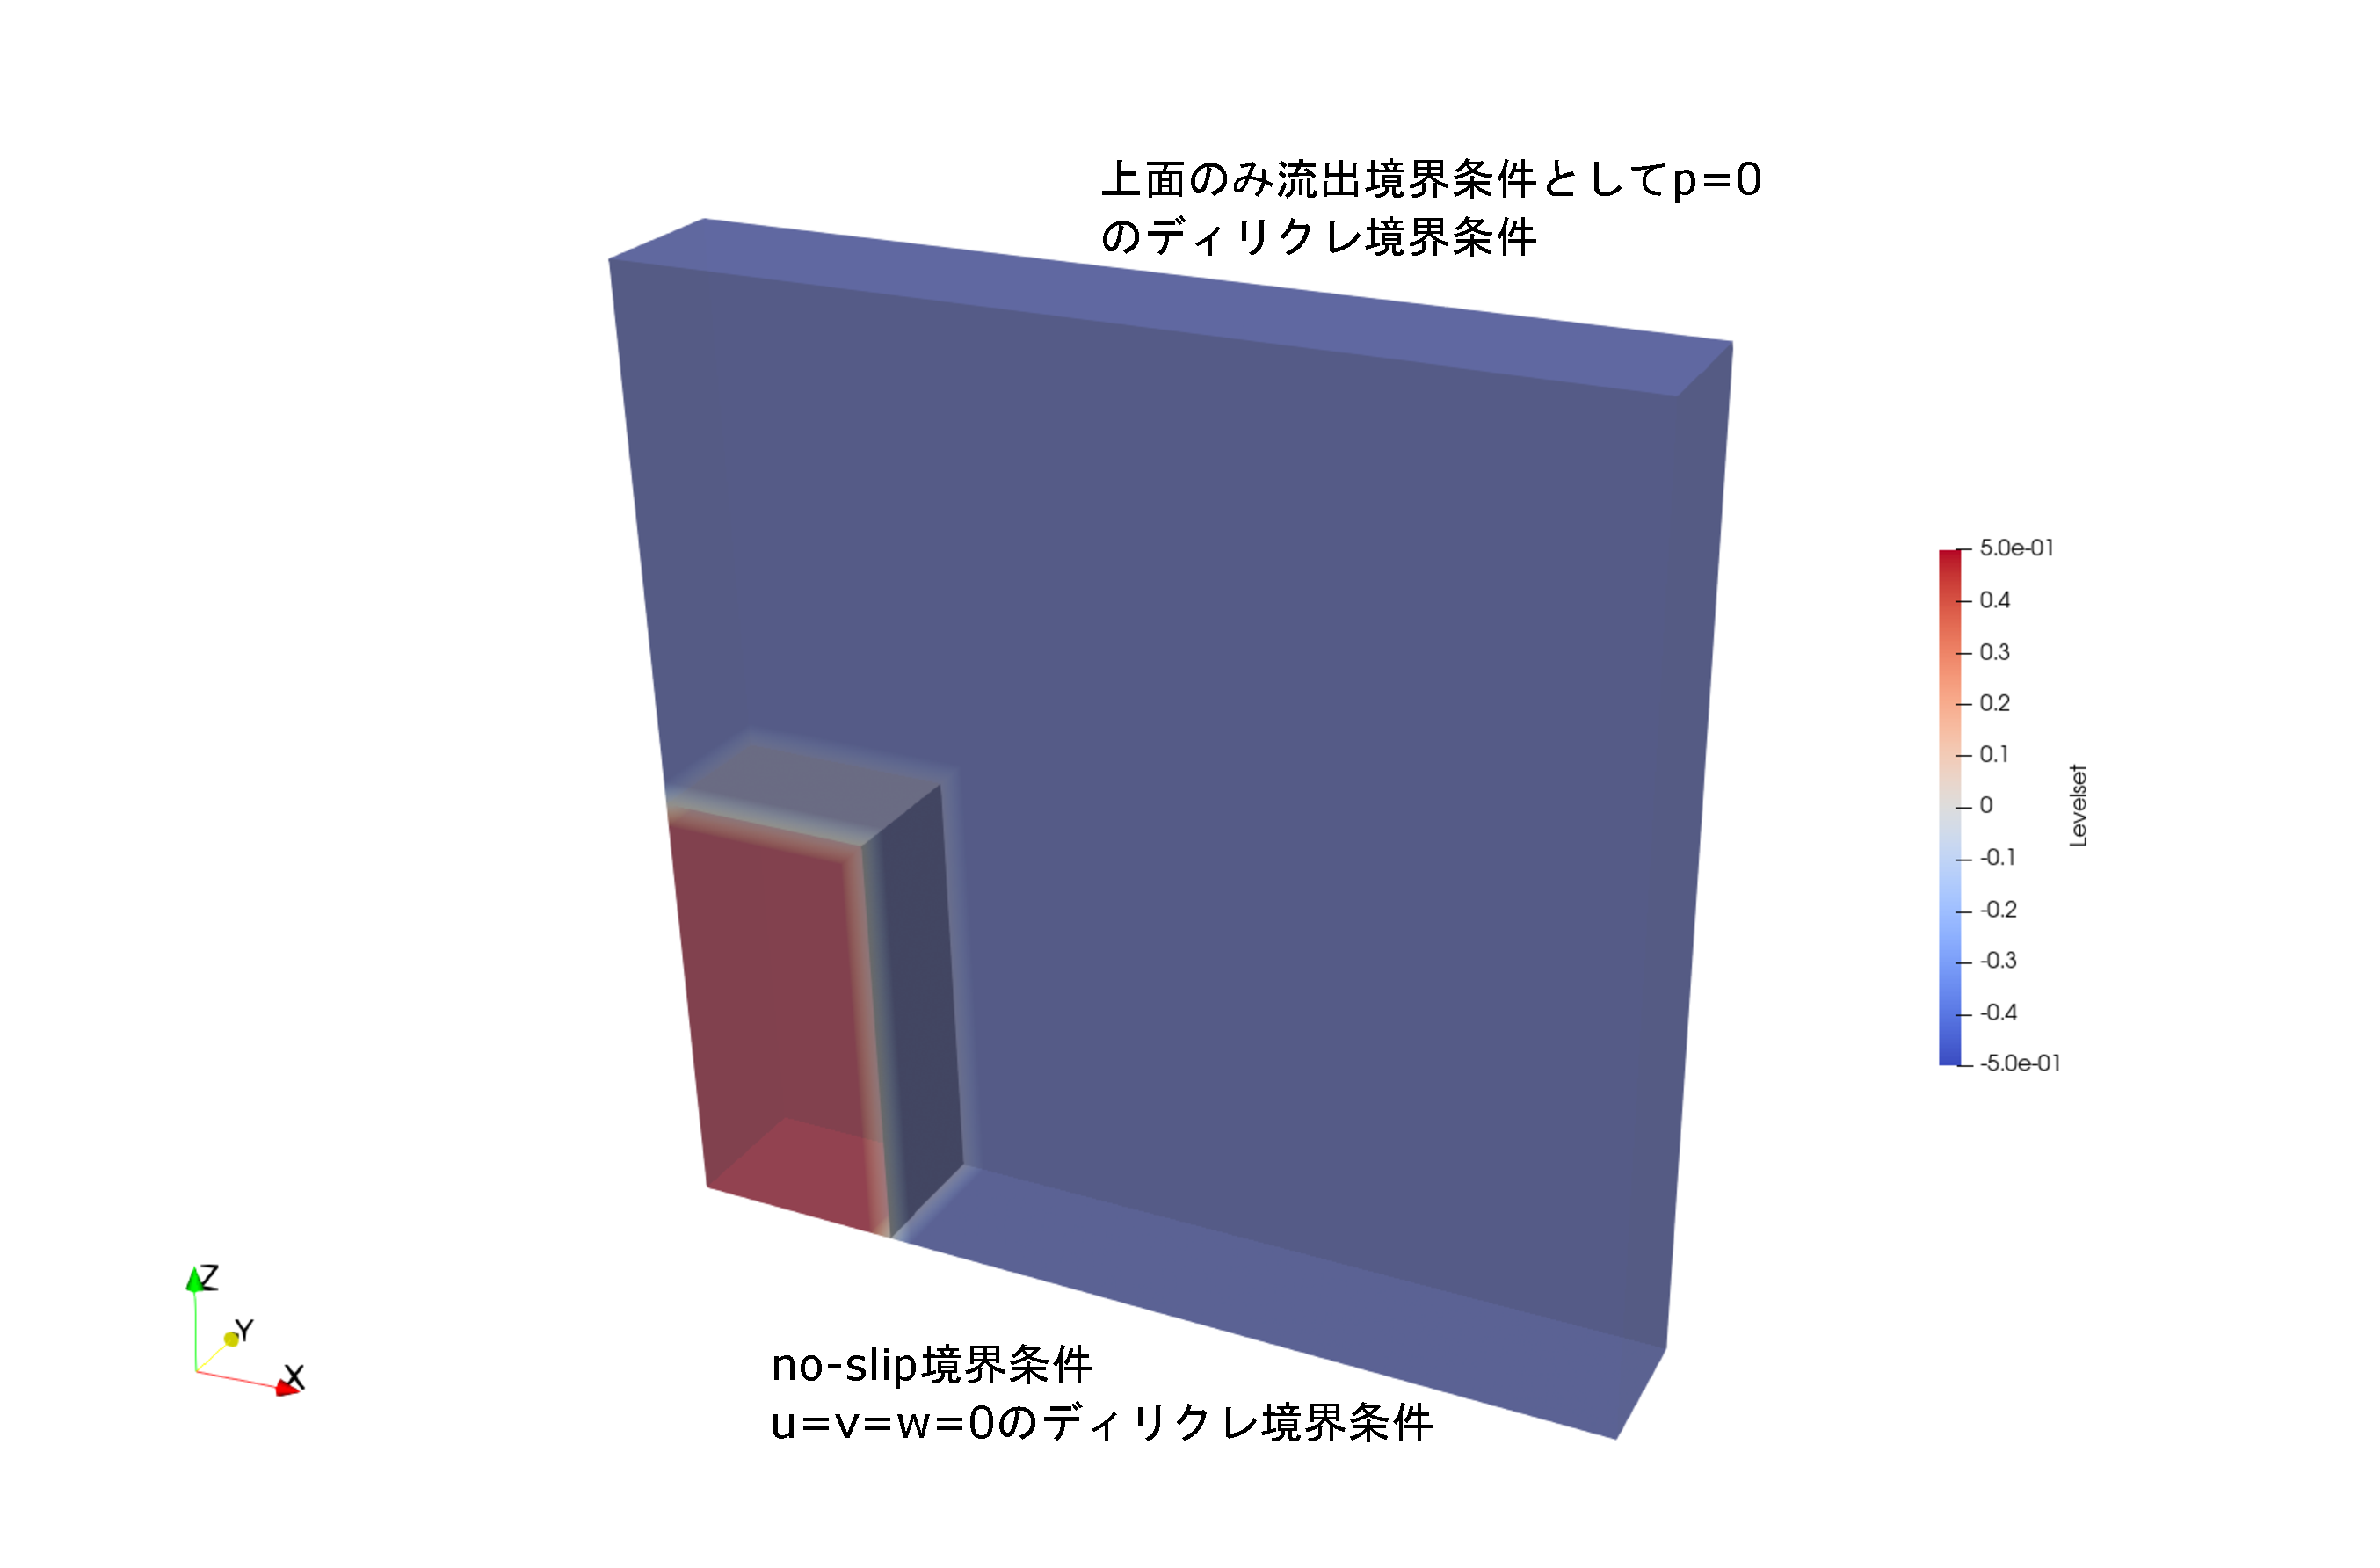
\includegraphics[width=6truecm]{pics/3d-sloshing/levelset_init.jpeg}
		\caption{3次元スロッシングのレベルセット関数($T=0$)}
		\label{fig:3d-sloshing-levelset_t0_3d}
	\end{minipage}
\end{figure}

スロッシングを起こすための水平加速度$f_{x}$は以下の式で与える。
\begin{equation}
	f_{x} = A \omega^2 \sin{\omega t}
\end{equation}
ここで、振幅$A=0.0093 \mathrm{m}$、角速度$\omega = 5.311 \mathrm{rad/s}$と設定した。

\newpage
\subsection{解析結果}
\subsubsection{メッシュ固定の場合の解析結果}

\begin{figure}[H]
	\centering
	\begin{minipage}[b]{0.19\columnwidth}
	    \centering
	    \includegraphics[width=3.5truecm]{pics/3d-sloshing/CN-dx0025/result_0010.jpeg}
	\end{minipage}
	\begin{minipage}[b]{0.19\columnwidth}
	    \centering
	    \includegraphics[width=3.5truecm]{pics/3d-sloshing/CN-dx0025/result_0012.jpeg}
	\end{minipage}
	\begin{minipage}[b]{0.19\columnwidth}
	    \centering
	    \includegraphics[width=3.5truecm]{pics/3d-sloshing/CN-dx0025/result_0014.jpeg}
	\end{minipage}
	\begin{minipage}[b]{0.19\columnwidth}
	    \centering
	    \includegraphics[width=3.5truecm]{pics/3d-sloshing/CN-dx0025/result_0016.jpeg}
	\end{minipage}
	\begin{minipage}[b]{0.19\columnwidth}
	    \centering
	    \includegraphics[width=3.5truecm]{pics/3d-sloshing/CN-dx0025/result_0018.jpeg}
	\end{minipage}
	\caption{スロッシングの結果($1.0\mathrm{s}$~$1.8\mathrm{s}$)}
	\label{fig:sloshing-result}
\end{figure}
\begin{figure}[H]
	\centering
	\begin{minipage}[b]{0.19\columnwidth}
	    \centering
	    \includegraphics[width=3.5truecm]{pics/3d-sloshing/CN-dx0025/result_0090.jpeg}
	\end{minipage}
	\begin{minipage}[b]{0.19\columnwidth}
	    \centering
	    \includegraphics[width=3.5truecm]{pics/3d-sloshing/CN-dx0025/result_0092.jpeg}
	\end{minipage}
	\begin{minipage}[b]{0.19\columnwidth}
	    \centering
	    \includegraphics[width=3.5truecm]{pics/3d-sloshing/CN-dx0025/result_0094.jpeg}
	\end{minipage}
	\begin{minipage}[b]{0.19\columnwidth}
	    \centering
	    \includegraphics[width=3.5truecm]{pics/3d-sloshing/CN-dx0025/result_0096.jpeg}
	\end{minipage}
	\begin{minipage}[b]{0.19\columnwidth}
	    \centering
	    \includegraphics[width=3.5truecm]{pics/3d-sloshing/CN-dx0025/result_0098.jpeg}
	\end{minipage}
	\caption{スロッシングの結果($9.0\mathrm{s}$~$9.8\mathrm{s}$)}
	\label{fig:sloshing-result}
\end{figure}

\begin{figure}[H]
    \centering
	\includegraphics[width=15truecm]{pics/3d-sloshing/height_time.pdf}
	\caption{スロッシング解析結果の左端の水位と参考文献\cite{Okamoto1992}, \cite{Sakuraba2001}との比較}
	\label{fig:3d-sloshing-result}
\end{figure}

参考までに、スロッシング解析では衝撃捕捉項(\ref{sec:fluid}章の式(\ref{fluid-GLS}))を入れない場合、6.0sあたりから計算が不安定になり発散しやすい傾向が見られた。
実際にALE法ではあるが、shock capturing項(衝撃捕捉項)を入れない場合と入れる場合の計算を比較し、入れない場合は6.0s過ぎた付近から計算が不安定となり、その後発散するが、入れた場合は安定的に計算ができた結果が報告されている\cite{Sakuraba1999}。

\newpage
\subsubsection{メッシュを移動させた場合の解析結果(ALE記述の実装の確認)}
ここでは、メッシュを移動させた場合の結果を示す。

\begin{figure}[H]
	\centering
	\begin{minipage}[b]{0.19\columnwidth}
	    \centering
	    \includegraphics[width=3.5truecm]{pics/3d-sloshing/ALE-dx0025/result_0010.jpeg}
	\end{minipage}
	\begin{minipage}[b]{0.19\columnwidth}
	    \centering
	    \includegraphics[width=3.5truecm]{pics/3d-sloshing/ALE-dx0025/result_0012.jpeg}
	\end{minipage}
	\begin{minipage}[b]{0.19\columnwidth}
	    \centering
	    \includegraphics[width=3.5truecm]{pics/3d-sloshing/ALE-dx0025/result_0014.jpeg}
	\end{minipage}
	\begin{minipage}[b]{0.19\columnwidth}
	    \centering
	    \includegraphics[width=3.5truecm]{pics/3d-sloshing/ALE-dx0025/result_0016.jpeg}
	\end{minipage}
	\begin{minipage}[b]{0.19\columnwidth}
	    \centering
	    \includegraphics[width=3.5truecm]{pics/3d-sloshing/ALE-dx0025/result_0018.jpeg}
	\end{minipage}
	\caption{スロッシングの結果($1.0\mathrm{s}$~$1.8\mathrm{s}$)}
	\label{fig:sloshing-result}
\end{figure}
\begin{figure}[H]
	\centering
	\begin{minipage}[b]{0.19\columnwidth}
	    \centering
	    \includegraphics[width=3.5truecm]{pics/3d-sloshing/ALE-dx0025/result_0090.jpeg}
	\end{minipage}
	\begin{minipage}[b]{0.19\columnwidth}
	    \centering
	    \includegraphics[width=3.5truecm]{pics/3d-sloshing/ALE-dx0025/result_0092.jpeg}
	\end{minipage}
	\begin{minipage}[b]{0.19\columnwidth}
	    \centering
	    \includegraphics[width=3.5truecm]{pics/3d-sloshing/ALE-dx0025/result_0094.jpeg}
	\end{minipage}
	\begin{minipage}[b]{0.19\columnwidth}
	    \centering
	    \includegraphics[width=3.5truecm]{pics/3d-sloshing/ALE-dx0025/result_0096.jpeg}
	\end{minipage}
	\begin{minipage}[b]{0.19\columnwidth}
	    \centering
	    \includegraphics[width=3.5truecm]{pics/3d-sloshing/ALE-dx0025/result_0098.jpeg}
	\end{minipage}
	\caption{スロッシングの結果($9.0\mathrm{s}$~$9.8\mathrm{s}$)}
	\label{fig:sloshing-result}
\end{figure}

\subsubsection{並列化解析結果}
並列化させた場合の結果と計算時間の比較を示す。

\begin{figure}[H]
    \centering
	\includegraphics[width=15truecm]{pics/3d-sloshing/CN-dx0010/Error-parallel.png}
	\caption{並列化エラー}
	\label{fig:3d-sloshing-error-parallel}
\end{figure}